\documentclass{beamer}

\usetheme[secheader]{Boadilla}
\setbeamertemplate{footline} {
  %\leavevmode%
  \hbox{%
  \begin{beamercolorbox}[wd=.5\paperwidth,ht=2.25ex,dp=1ex,left]{author in head/foot}%
    \usebeamerfont{author in head/foot}\hspace*{2ex}\insertshortauthor~~(adraeger@cern.ch)
  \end{beamercolorbox}%
  \begin{beamercolorbox}[wd=.5\paperwidth,ht=2.25ex,dp=1ex,right]{date in head/foot}%
    \usebeamerfont{date in head/foot}\insertshorttitle,~
    \insertshortdate{}\hspace*{1em}
    \insertframenumber{} / \inserttotalframenumber\hspace*{2ex}
  \end{beamercolorbox}}%
  \vskip0pt%
}
\beamertemplatenavigationsymbolsempty

\usepackage[percent]{overpic}
\usepackage{tikz}
\usetikzlibrary{positioning,fit,shapes.arrows,shapes.geometric,shapes.misc,shapes.multipart,calc,shadows}
\tikzstyle{every picture}+=[remember picture]
\usepackage{booktabs}
\usepackage{graphicx}
\usepackage{rotating}
\usepackage{wasysym}
\graphicspath{{../../logo/}{figures/}{../../graphic-common/}}

\usepackage{amsmath}
\usepackage{cancel}
\usepackage{xspace}
\usepackage{xcolor}

% editing
\newcommand{\todo}[1]{\textcolor{red}{{\textbf{TODO: }\textit{#1}}}\xspace}
\newcommand{\fixme}[1]{\textcolor{red}{{\textbf{FIXME: }\textit{#1}}}}

% helpers
\newcommand{\emptybox}[1]{\parbox[c][#1]{0pt}{}}

% boxes
\newcommand{\cfbox}[2]{{\color{#1}\fbox{\normalcolor#2}}}

% Sectioning
\newcommand{\qsec}[1]{Section~\ref{#1}}
\newcommand{\qfig}[1]{Fig.~\ref{#1}}
\newcommand{\qtab}[1]{Table~\ref{#1}}
\newcommand{\qeq}[1]{\eqref{#1}}

% Particles
\newcommand{\W}{\ensuremath{\text{W}}\xspace}
\newcommand{\Z}{\ensuremath{\text{Z}}\xspace}

% Processes
\newcommand{\ZInv}{\ensuremath{\text{Z}\rightarrow\nu\bar{\nu}}\xspace}
\newcommand{\ZInvJets}{\ensuremath{\text{Z}\rightarrow\nu\bar{\nu}\,+\,\text{jets}}\xspace}
\newcommand{\Zmumu}{\ensuremath{\text{Z}\rightarrow\mu\bar{\mu}}\xspace}
\newcommand{\Zll}{\ensuremath{\text{Z}\rightarrow\text{ll}}\xspace}
\newcommand{\Zee}{\ensuremath{\text{Z}\rightarrow\text{ee}}\xspace}
\newcommand{\ttbar}{\ensuremath{\text{t}\bar{\text{t}}}\xspace}
\newcommand{\bbbar}{\ensuremath{\text{b}\bar{\text{b}}}\xspace}
\newcommand{\ccbar}{\ensuremath{\text{c}\bar{\text{c}}}\xspace}
\newcommand{\wpj}{\ensuremath{\text{W}+\text{jets}}\xspace}
\newcommand{\photonJet}{\ensuremath{\gamma+\text{jet}}\xspace}
\newcommand{\photonJets}{\ensuremath{\gamma+\text{jets}}\xspace}
\newcommand{\ZJet}{\ensuremath{\text{Z}+\text{jet}}\xspace}
\newcommand{\ZJets}{\ensuremath{\text{Z}+\text{jets}}\xspace}
\newcommand{\photonZJet}{\ensuremath{\text{photon}/Z+\text{jet}}\xspace}
\newcommand{\muonJets}{\ensuremath{\mu+\text{jets}}\xspace}
\newcommand{\hadtau}{\ensuremath{\tau_{Had}}\xspace}
\newcommand{\wtotau}{\ensuremath{\text{W}\rightarrow\tau}\xspace}
\newcommand{\wtotautomu}{\ensuremath{\text{W}\rightarrow\tau\rightarrow\mu}\xspace}
\newcommand{\wtohadtau}{\ensuremath{\text{W}\rightarrow\tau_{Had}}\xspace}
\newcommand{\wtomu}{\ensuremath{\text{W}\rightarrow\mu}\xspace}
\newcommand{\wtolnu}{\ensuremath{\text{W}\rightarrow \text{l}\nu}\xspace}
\newcommand{\wtoe}{\ensuremath{\text{W}\rightarrow\text{e}}\xspace}
% Units
\newcommand{\tev}{\ensuremath{\;\text{Te}\kern-0.06667em\text{V}}\xspace}
\newcommand{\gev}{\ensuremath{\;\text{Ge}\kern-0.06667em\text{V}}\xspace}
\newcommand{\gevbrackets}{\ensuremath{\;[\text{Ge}\kern-0.06667em\text{V}]}\xspace}
\newcommand{\mev}{\ensuremath{\;\text{Me}\kern-0.06667em\text{V}}\xspace}
\newcommand{\kev}{\ensuremath{\;\text{ke}\kern-0.06667em\text{V}}\xspace}
\newcommand{\ev}{\ensuremath{\;\text{e}\kern-0.06667em\text{V}}\xspace}
\newcommand{\km}{\ensuremath{\;\text{km}}\xspace}
\newcommand{\m}{\ensuremath{\;\text{m}}\xspace}
\newcommand{\cm}{\ensuremath{\;\text{cm}}\xspace}
\newcommand{\mm}{\ensuremath{\;\text{mm}}\xspace}
\newcommand{\mum}{\ensuremath{\;\mu\text{m}}\xspace}
\newcommand{\hour}{\ensuremath{\;\text{h}}\xspace}
\newcommand{\second}{\ensuremath{\;\text{s}}\xspace}
\newcommand{\ns}{\ensuremath{\;\text{ns}}\xspace}
\newcommand{\kg}{\ensuremath{\;\text{kg}}\xspace}
\newcommand{\tons}{\ensuremath{\;\text{t}}\xspace}
\newcommand{\tesla}{\ensuremath{\;\text{T}}\xspace}
\newcommand{\kelvin}{\ensuremath{\;\text{K}}\xspace}
\newcommand{\nbinv}{\ensuremath{\;\text{nb}^{-1}}\xspace}
\newcommand{\pbinv}{\ensuremath{\;\text{pb}^{-1}}\xspace}
\newcommand{\fbinv}{\ensuremath{\;\text{fb}^{-1}}\xspace}
\newcommand{\pb}{\ensuremath{\;\text{pb}}\xspace}
\newcommand{\fb}{\ensuremath{\;\text{fb}}\xspace}
\newcommand{\mb}{\ensuremath{\;\text{mb}}\xspace}
\newcommand{\Hz}{\ensuremath{\;\text{Hz}}\xspace}

\newcommand{\gevnospace}{\ensuremath{\text{Ge}\kern-0.06667em\text{V}}\xspace}
\newcommand{\tevnospace}{\ensuremath{\text{Te}\kern-0.06667em\text{V}}\xspace}

% Quantities
\newcommand{\et}{\ensuremath{E_{\text{T}}}\xspace}
\newcommand{\met}{\ensuremath{\slash\mkern-12mu{E}_{\text{T}}}\xspace}
\newcommand{\metvec}{\ensuremath{\slash\mkern-12mu{\vec{E}}_{\text{T}}}\xspace}
\newcommand{\jetht}{\ensuremath{H_{\text{T}}}\xspace}
\newcommand{\mht}{\ensuremath{\slash\mkern-12mu{H}_{\text{T}}}\xspace}
\newcommand{\HT}{\ensuremath{H_{\text{T}}}\xspace}
\newcommand{\MHT}{\ensuremath{\slash\mkern-12mu{H}_{\text{T}}}\xspace}
\newcommand{\pt}{\ensuremath{p_{\text{T}}}\xspace}
\newcommand{\ptsup}[1]{\ensuremath{p^{#1}_{\text{T}}}\xspace}
\newcommand{\ptvec}{\ensuremath{\vec{p}_{\text{T}}}\xspace}
\newcommand{\ptvecsup}[1]{\ensuremath{\vec{p}^{#1}_{\text{T}}}\xspace}
\newcommand{\pti}[1]{\ensuremath{p_{\text{T},#1}}\xspace}
\newcommand{\ptivec}[1]{\ensuremath{\vec{p}_{\text{T},#1}}\xspace}
\newcommand{\ptjeti}[1]{\ensuremath{p^{\text{jet#1}}_{\text{T}}}\xspace}
\newcommand{\ptsub}[1]{\ensuremath{p_{\text{T},#1}}\xspace}
\newcommand{\ptvecsub}[1]{\ensuremath{\vec{p}_{\text{T},#1}}\xspace}
\newcommand{\ptdijet}{\ensuremath{p^{\text{dijet}}_{\text{T}}}\xspace}
\newcommand{\ptave}{\ensuremath{p^{\text{ave}}_{\text{T}}}\xspace}
\newcommand{\ptavemin}{\ensuremath{p^{\text{ave,min}}_{\text{T}}}\xspace}
\newcommand{\ptavemax}{\ensuremath{p^{\text{ave,max}}_{\text{T}}}\xspace}
\newcommand{\ptgen}{\ensuremath{p^{\text{gen}}_{\text{T}}}\xspace}
\newcommand{\ptgenave}{\ensuremath{p^{\text{gen,ave}}_{\text{T}}}\xspace}
\newcommand{\ptgenrel}{\ensuremath{p^{\text{gen,rel}}_{\text{T,3}}}\xspace}
\newcommand{\ptgeni}[1]{\ensuremath{p^{\text{gen}}_{\text{T},#1}}\xspace}
\newcommand{\pthat}{\ensuremath{\hat{p}_{\text{T}}}\xspace}
\newcommand{\pthatmin}{\ensuremath{\hat{p}^{\text{min}}_{\text{T}}}\xspace}
\newcommand{\pthatmax}{\ensuremath{\hat{p}^{\text{max}}_{\text{T}}}\xspace}
\newcommand{\pttrue}{\ensuremath{p^{\text{true}_{}}_{\text{T}}}\xspace}
\newcommand{\pttruei}[1]{\ensuremath{p^{\text{true}_{}}_{\text{T,}#1}}\xspace}
\newcommand{\ptmeas}{\ensuremath{p^{\text{meas}_{}}_{\text{T}}}\xspace}
\newcommand{\ptmeasi}[1]{\ensuremath{p^{\text{meas}_{}}_{\text{T,}#1}}\xspace}
\newcommand{\ptreco}{\ensuremath{p^{\text{reco}_{}}_{\text{T}}}\xspace}
\newcommand{\ptrel}{\ensuremath{\alpha}\xspace}
\newcommand{\ptrelmax}{\ensuremath{\alpha_{\text{max}}}\xspace}
\newcommand{\ptmin}{\ensuremath{p^{\text{min}_{}}_{\text{T}}}\xspace}
\newcommand{\ptmax}{\ensuremath{p^{\text{max}_{}}_{\text{T}}}\xspace}
\newcommand{\ptcalo}{\ensuremath{p^{\text{calo}_{}}_{\text{T}}}\xspace}
\newcommand{\ptcaloi}[1]{\ensuremath{p^{\text{calo}_{}}_{\text{T},#1}}\xspace}
\newcommand{\ptparticle}{\ensuremath{p^{\text{particle}_{}}_{\text{T}}}\xspace}
\newcommand{\ptparton}{\ensuremath{p^{\text{parton}_{}}_{\text{T}}}\xspace}
\newcommand{\ptref}{\ensuremath{p^{\text{ref}_{}}_{\text{T}}}\xspace}
\newcommand{\ppgen}{\ensuremath{p^{\text{gen}}_{||}}\xspace}
\newcommand{\ppgeni}[1]{\ensuremath{p^{\text{gen}}_{||,#1}}\xspace}
\newcommand{\pp}{\ensuremath{p_{||}}\xspace}
\newcommand{\ppi}[1]{\ensuremath{p_{||,#1}}\xspace}
\newcommand{\ppirel}[1]{\ensuremath{p^{\text{rel}}_{||,#1}}\xspace}
\newcommand{\etajeti}[1]{\ensuremath{\eta^{\text{jet#1}}}\xspace}
\newcommand{\etamin}{\ensuremath{\eta^{\text{min}}}\xspace}
\newcommand{\etamax}{\ensuremath{\eta^{\text{max}}}\xspace}
\newcommand{\fasym}{\ensuremath{f_{\text{Asym}}}\xspace}
\newcommand{\fasymdata}{\ensuremath{f^{\text{Data}}_{\text{Asym}}}\xspace}
\newcommand{\fasymmc}{\ensuremath{f^{\text{MC}}_{\text{Asym}}}\xspace}
\newcommand{\fresp}{\ensuremath{f_{\text{Resp}}}\xspace}
\newcommand{\alphat}{\ensuremath{\alpha_{\text{T}}}\xspace}
\newcommand{\resp}{\ensuremath{\mathcal{R}}\xspace}
\newcommand{\respmctruth}{\ensuremath{\mathcal{R}_{\text{MC}}}\xspace}
\newcommand{\sigmatruth}{\ensuremath{\sigma_{\text{MC}}}\xspace}
\newcommand{\asym}{\ensuremath{\mathcal{A}}\xspace}
\newcommand{\datasimratio}{\ensuremath{\rho}\xspace}
\newcommand{\NJets}{\ensuremath{N_{\text{jets}}}\xspace}
\newcommand{\BTags}{\ensuremath{B_{\text{tags}}}\xspace}
\newcommand{\Mass}[1]{\ensuremath{\text{M}_{\text{#1}}\xspace}}
\newcommand{\mass}[1]{\ensuremath{\text{m}_{\text{#1}}\xspace}}
\newcommand{\mtw}{\ensuremath{m_{T}(\text{W})\xspace}}
\newcommand{\mt}{\ensuremath{m_{T}\xspace}}

\newcommand{\deltaphi}{\ensuremath{\Delta\phi}\xspace}
\newcommand{\mindeltaphi}{\ensuremath{\Delta\phi_{N}^{min}}\xspace}
\newcommand{\dphin}{\ensuremath{\Delta \hat\phi_{\mathrm{min}}}\xspace}
\newcommand{\deltaR}{\ensuremath{\Delta R}\xspace}

% Symbols
\newcommand{\dif}[1]{\ensuremath{\text{d}#1}\xspace}
\newcommand{\e}{\,\text{e}}
\newcommand{\nup}[1]{$^{\text{\scriptsize #1}}$}
\newcommand{\dgr}{\ensuremath{\,^{\circ}}}
\newcommand{\mean}[1]{\ensuremath{\langle#1\rangle}}
\newcommand{\gqq}[1]{\ensuremath{\glqq#1\grqq}}
\newcommand{\rarr}{\ensuremath{\rightarrow}\xspace}

% Words and characters
\newcommand{\sm}{SM\xspace}
\newcommand{\diagonalsout}[1]{\ensuremath{\cancel{\text{#1}}}}
\newcommand{\genjet}{GenJet\xspace}
\newcommand{\genjets}{GenJets\xspace}
\newcommand{\calojet}{CaloJet\xspace}
\newcommand{\calojets}{CaloJets\xspace}
\newcommand{\window}[2]{\ensuremath{#1-#2\,\sigma}}
\newcommand{\windowinf}[1]{\ensuremath{#1\,\sigma - \infty}}
\newcommand{\pythia}{\textsc{Pythia}\xspace}
\newcommand{\pythiasix}{\textsc{Pythia6}\xspace}
\newcommand{\herwigpp}{\textsc{Herwig++}\xspace}
\newcommand{\herwig}{\textsc{Herwig}\xspace}
\newcommand{\madgraph}{\textsc{Madgraph}\xspace}
\newcommand{\CL}{C.\,L.\xspace}

% Jet related
\newcommand{\antikt}{anti-$k_{\text{T}}$\xspace}

% SUSY related
\newcommand{\susy}{SUSY\xspace}
\newcommand{\mssm}{MSSM\xspace}
\newcommand{\cmssm}{cMSSM\xspace}
\newcommand{\pmssm}{pMSSM\xspace}
\newcommand{\lsp}{LSP\xspace}
\newcommand{\mzero}{\ensuremath{m_{0}}\xspace}
\newcommand{\monehalf}{\ensuremath{m_{1/2}}\xspace}
\newcommand{\squark}{\ensuremath{\tilde{q}}\xspace}
\newcommand{\gluino}{\ensuremath{\tilde{g}}\xspace}
\newcommand{\msquark}{\ensuremath{m_{\tilde{q}}}\xspace}
\newcommand{\mgluino}{\ensuremath{m_{\tilde{g}}}\xspace}
\newcommand{\mneutralino}{\ensuremath{m_{\tilde{\chi}^{0}}}\xspace}
\newcommand{\tanbeta}{\ensuremath{\tan\beta}\xspace}
\newcommand{\stau}{\ensuremath{\tilde{\tau}}\xspace}
\newcommand{\neutralino}{\ensuremath{\tilde{\chi}^{0}}\xspace}

% Higgs related
\newcommand{\phitobb}{\ensuremath{\Phi\rightarrow\text{b}\bar{\text{b}}}\xspace}
\newcommand{\mhiggs}{\ensuremath{m_{\text{H}}}\xspace}
\newcommand{\mA}{\ensuremath{m_{\text{A}}}\xspace}
\newcommand{\mh}{\ensuremath{m_{\text{h}}}\xspace}
\newcommand{\mH}{\ensuremath{m_{\text{H}}}\xspace}
\newcommand{\mPhi}{\ensuremath{M_{\Phi}}\xspace}
\newcommand{\btageff}{\ensuremath{\epsilon(\text{b-tag})}\xspace}
\newcommand{\mjj}{\ensuremath{M_{12}}\xspace}
\newcommand{\xjjj}{\ensuremath{X_{123}}\xspace}
\newcommand{\mhmax}{\ensuremath{m^{\text{max}}_{h}}\xspace}


% Abbrevations
\newcommand{\etc}{etc.\ }
\newcommand{\wrt}{w.\,r.\,t.\ }
\newcommand{\cf}{cf.\ }
\newcommand{\ie}{i.\,e.\ }
\newcommand{\siehe}{s.\ }
\newcommand{\zb}{z.\,B.\ }
\newcommand{\ca}{ca.\ }
\newcommand{\eg}{e.\,g.\ }
\newcommand{\vs}{vs.\ }
\newcommand{\NB}{N.\,B.\xspace}

% Misc
\newcommand{\solidline}[1]{\textcolor{#1}{---}}
\newcommand{\dashedline}[1]{\textcolor{#1}{- -}}
\newcommand{\opencircle}[1]{\textcolor{#1}{$\circ$}}
\newcommand{\solidcircle}[1]{\textcolor{#1}{$\bullet$}}
\newcommand{\solidsquare}[1]{\textcolor{#1}{\small $\blacksquare$}}
\newcommand{\solidtriangle}[1]{\textcolor{#1}{\small $\blacktriangle$}}
\newcommand{\opensquare}[1]{\textcolor{#1}{\small $\square$}}
\newcommand{\opentriangle}[1]{\textcolor{#1}{\small $\triangle$}}
\newcommand{\opendiamond}[1]{\textcolor{#1}{\small $\diamond$}}
\newcommand{\greencheck}{\textcolor{beamerGreen}{\ensuremath{\checkmark}}\xspace}
\newcommand{\bibbullet}{\includegraphics[width=1em]{../../graphic-common/eyeCandy/freehand-book.png}}

% Colours
\definecolor{beamerGreen}{rgb}{0,0.6,0}
\definecolor{darkGreen}{rgb}{0,0.6,0}
\definecolor{beamerYellow}{rgb}{1.,0.745,0}
\definecolor{gray}{rgb}{0.4,0.4,0.4}
\definecolor{darkgreen}{RGB}{000,100,000}
\definecolor{kGreen2}{RGB}{000,153,000}
\definecolor{theme_blue}{RGB}{051,051,178}
\definecolor{theme_blue_light}{HTML}{ADADE0}

\newcommand{\blue}[1]{\textcolor{blue}{#1}}
\newcommand{\themeblue}[1]{\textcolor{theme_blue}{#1}}
\newcommand{\red}[1]{\textcolor{red}{#1}}
\newcommand{\orange}[1]{\textcolor{orange}{#1}}
\newcommand{\green}[1]{\textcolor{green}{#1}}
\newcommand{\yellow}[1]{\textcolor{yellow}{#1}}
\newcommand{\white}[1]{\textcolor{white}{#1}}
\newcommand{\grey}[1]{\textcolor{gray}{#1}}
\newcommand{\link}[2]{\href{#1}{\textcolor{theme_blue}{\underline{#2}}}}

% Libre-Office colours
\definecolor{oochart2}{HTML}{FF420E}  % orange
\definecolor{oochart7}{HTML}{314004}  % dark green
\definecolor{oochart11}{RGB}{197,001,012} % dark red
\definecolor{oochart12}{RGB}{001,132,209} % light blue


% ROOT colors
\definecolor{kBlack}{HTML}{000000}
\definecolor{kRed}{HTML}{FF0000}
\definecolor{kRedUp2}{HTML}{6B0C0C}
\definecolor{kYellow}{HTML}{FEFE12}
\definecolor{kBlue}{HTML}{0000FF}
\definecolor{kOrange}{HTML}{FFCC00}
\definecolor{kGreen}{HTML}{59D454}
\definecolor{kGreenUp2}{HTML}{009900}
\definecolor{kMagenta}{HTML}{FF00FF}
\definecolor{kCyan}{HTML}{00FFFF}

% Colored symbols
\newcommand{\mysquare}[1][black]{\scriptsize\textcolor{#1}{\ensuremath\blacksquare}}
\newcommand{\mycirc}[1][black]{\scriptsize\textcolor{#1}{\ensuremath\bullet}}
\newcommand{\mylozenge}[1][black]{\small\textcolor{#1}{\ensuremath\blacklozenge}}
\newcommand{\mytriangle}[1][black]{\small\textcolor{#1}{\ensuremath\blacktriangle}}
\newcommand{\mydtriangle}[1][black]{\small\textcolor{#1}{\ensuremath\blacktriangledown}}
\newcommand{\mystar}[1][black]{\Large\textcolor{#1}{\ensuremath\star}} %% or \bigstar


% Title etc
\title[CMSDAS 2015 BARI]{Search for New Physics\\ in the Multijet and \met Final State}
\subtitle{Long Exercise, CMSDAS 2015, Bari}
\author[Arne-Rasmus~Dr\"ager]{\underline{Arne-Rasmus~Dr\"ager}\inst{1}, Dr.~Tai~Sakuma\inst{2}}
\institute{
  \inst{1} University of Hamburg, \inst{2}  University of Bristol (GB)
}
\date{January 2015}

% \author[Matthias~Schr\"oder]{\underlineArne-Rasmus~Dr\"ager}\inst{1},Dr.~Tai~Sakuma\inst{2}}
% \institute{
%   \inst{1} University of Hamburg, \inst{1} University of Bristol (GB)\inst{2}
% }

% pdflatex packages
\hypersetup{bookmarks=true}
\hypersetup{pdftitle={CMSDAS 2015 BARI}}
\hypersetup{pdfauthor={Arne-Rasmus~Dr\"ager}}
\hypersetup{bookmarks=true}


\begin{document}
% ==================================================
% --------------------------------------------------
\begin{frame}
  \titlepage
\end{frame}

% --------------------------------------------------

\section{Supersymmetry}
% --------------------------------------------------
\begin{frame}
  \frametitle{What We Know}
  \begin{columns}
    \begin{column}{0.49\textwidth}
      \centering
      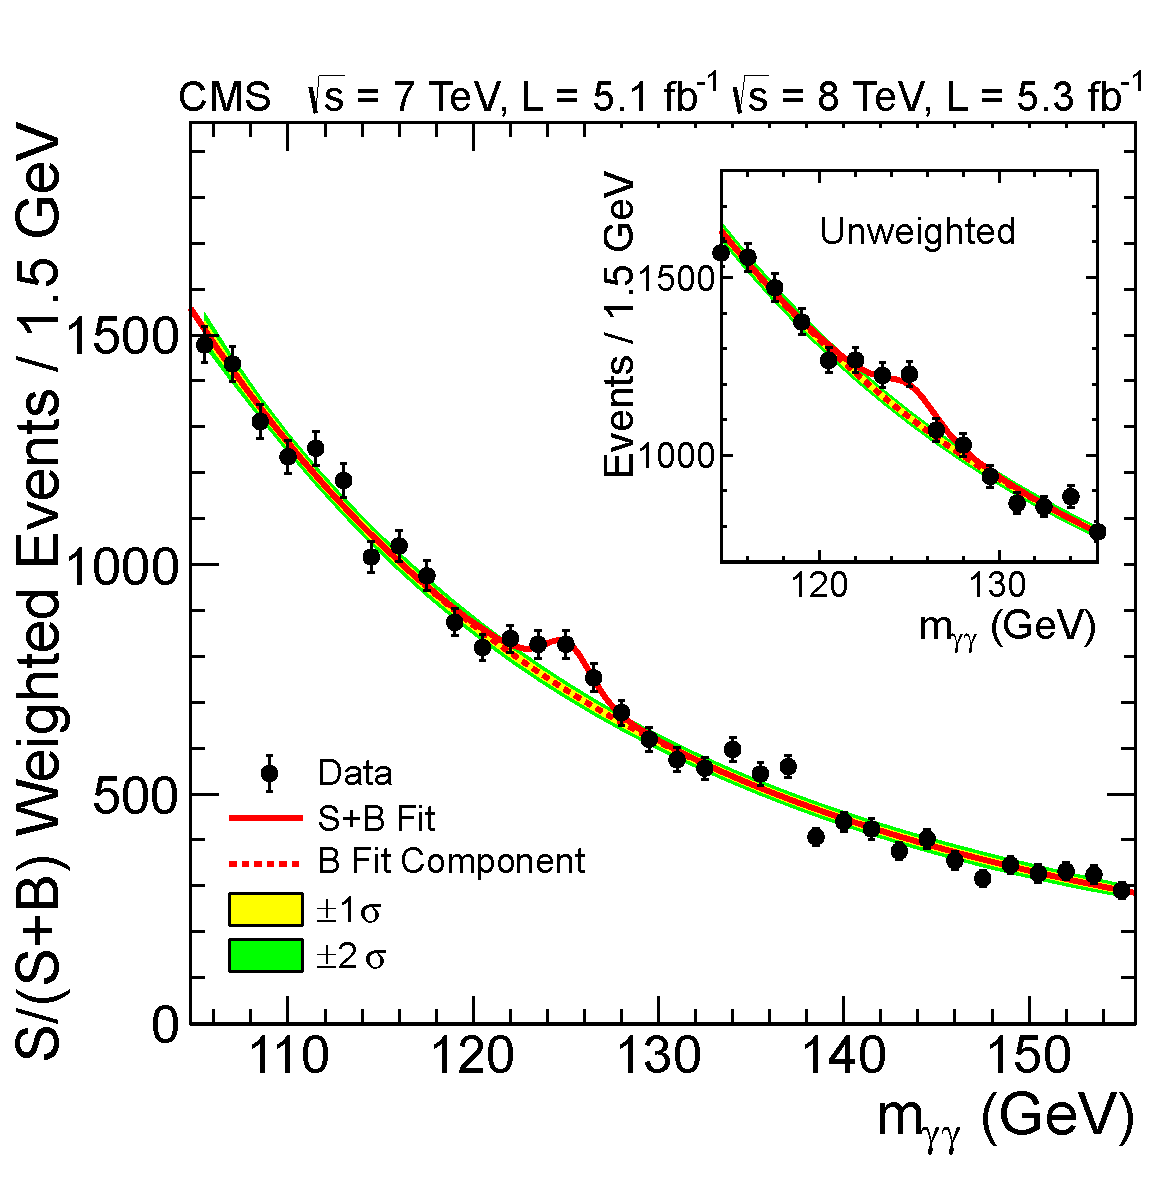
\includegraphics[width=\textwidth]{figures/fig3.pdf}\\
    \end{column}
    \begin{column}{0.51\textwidth}
      \centering
      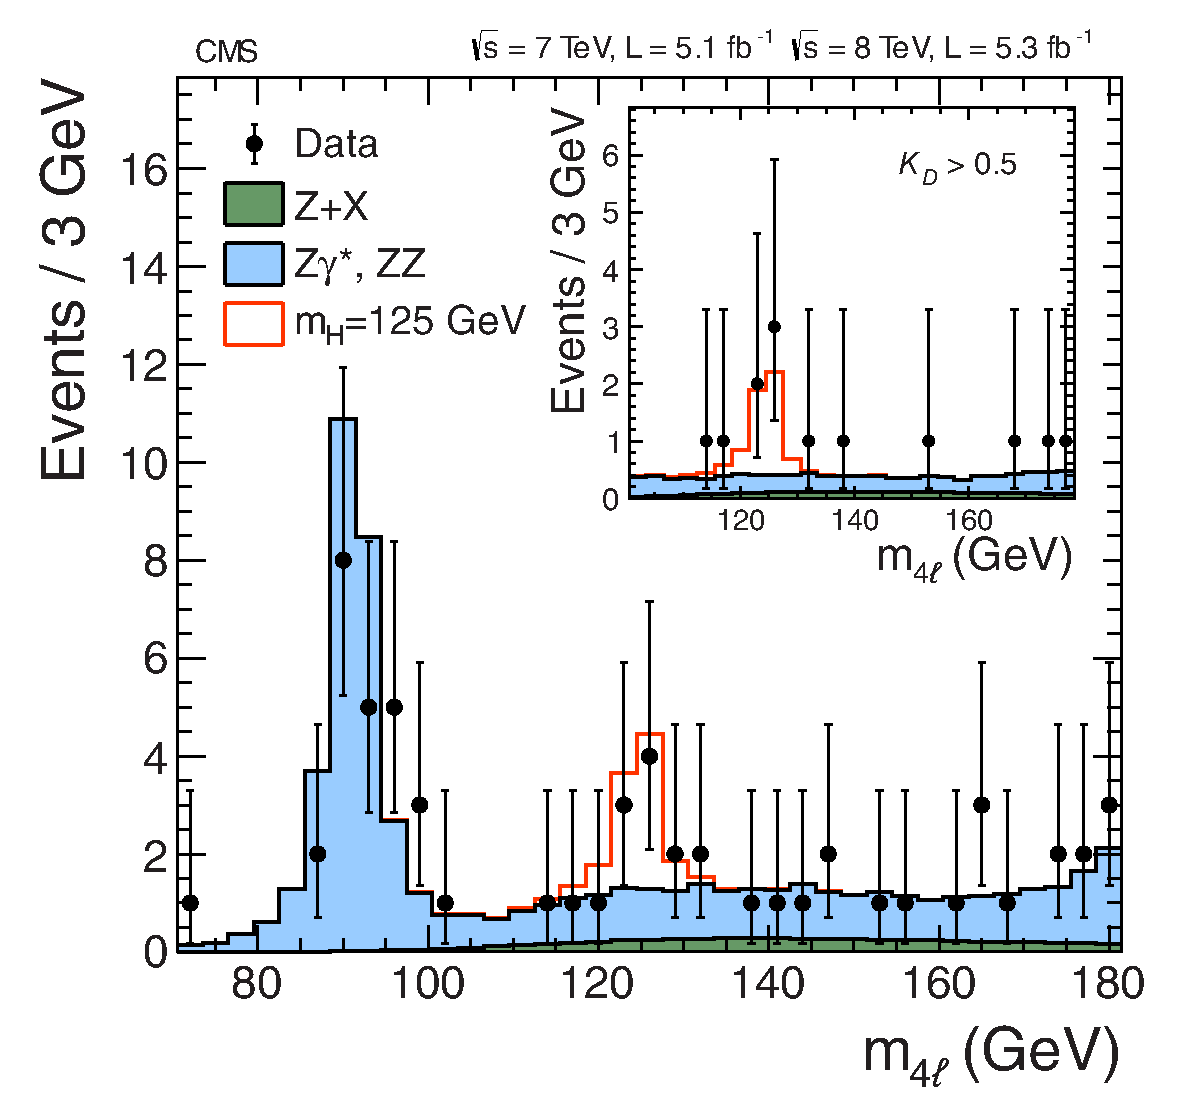
\includegraphics[width=\textwidth]{figures/fig4.pdf}\\
    \end{column}
  \end{columns}
  \begin{block}{}
    \centering
    \textbf{The Standard Model is completed \checkmark}
  \end{block}
\end{frame}

% ---------------------------------------------------------------------------------
\begin{frame}
  \frametitle{What We Don't Know}
  \begin{columns}
    \begin{column}{0.5\textwidth}
      \centering
      \visible<2->{
        
\includegraphics[height=2.5cm]{figures/leonard.jpeg}
      }
    \end{column}
    \begin{column}{0.5\textwidth}
      \visible<3->{
        \centering
        
\includegraphics[height=2.5cm]{figures/sheldon.jpg}
      }
    \end{column}
  \end{columns}
  \vskip0.3cm
  \begin{columns}
    \begin{column}{0.5\textwidth}
      \visible<2->{
        \centering
        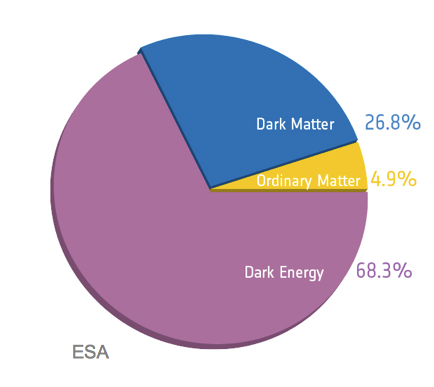
\includegraphics[width=0.55\textwidth]{susy/PlanckUniverse.png}\\
      }
    \end{column}
    \begin{column}{0.5\textwidth}
      \visible<3->{
        \centering
        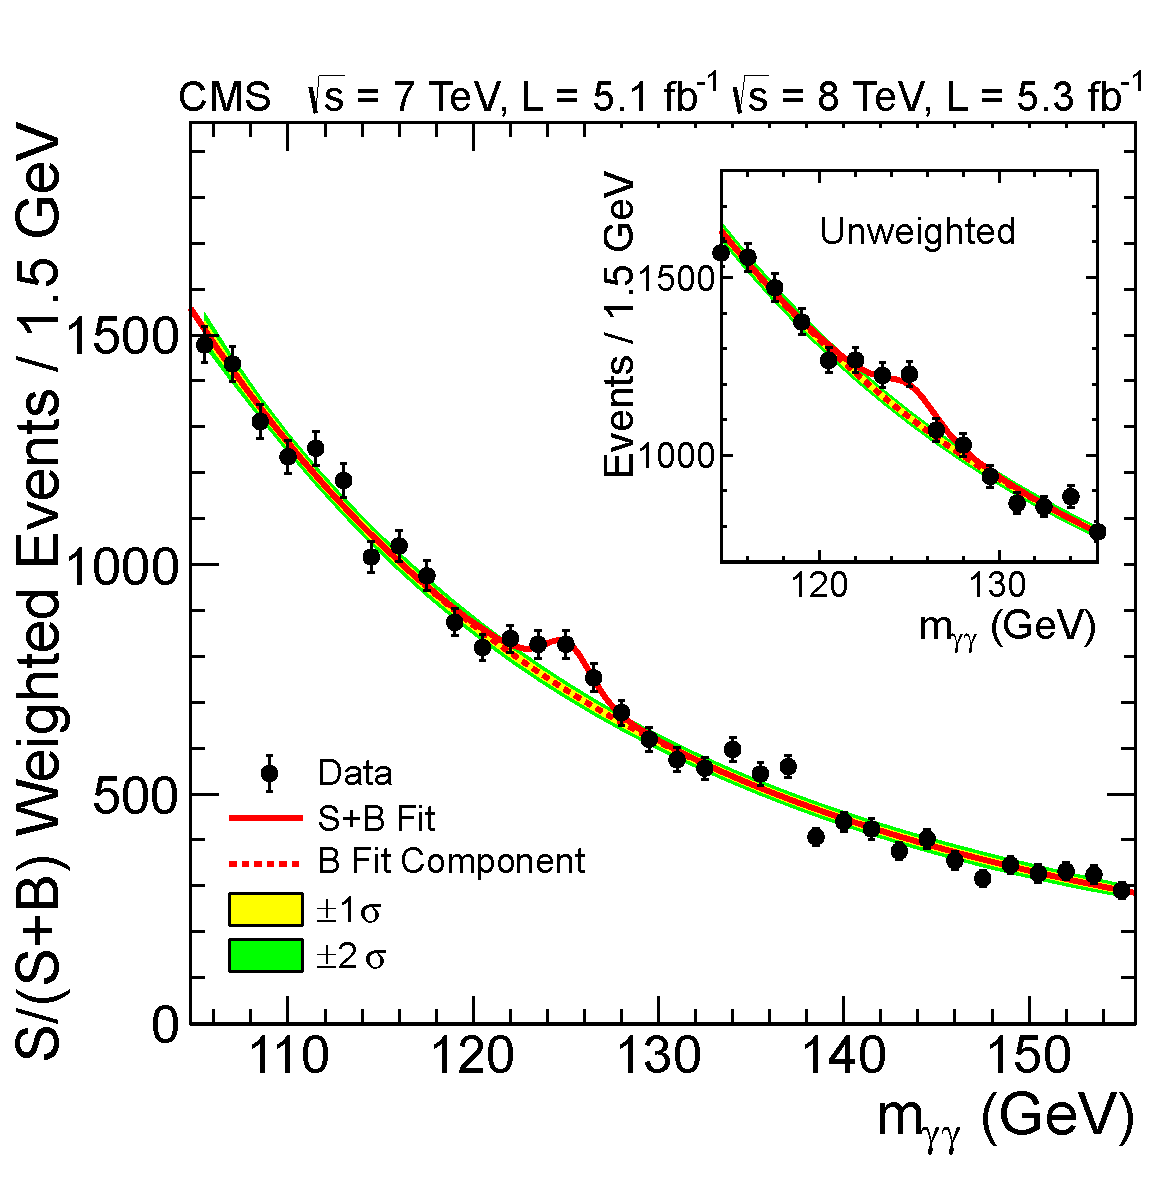
\includegraphics[width=0.4\textwidth]{figures/fig3.pdf}
        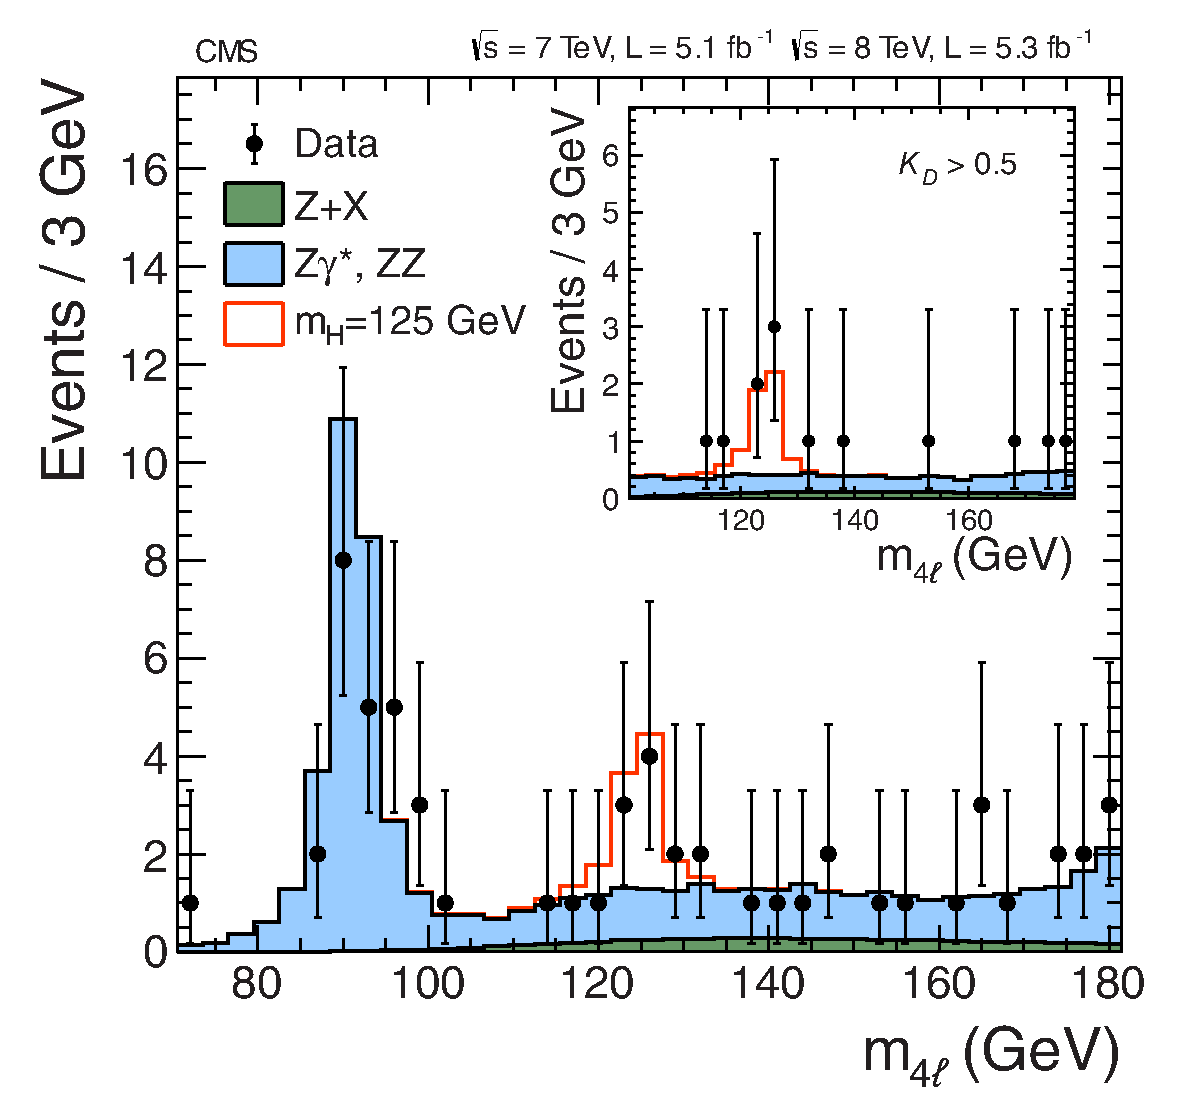
\includegraphics[width=0.42\textwidth]{figures/fig4.pdf}
      }
    \end{column}
  \end{columns}
  \begin{columns}
    \begin{column}{0.5\textwidth}
      \visible<2->{
        \centering
        \structure{What are those 95\%?}
      }
    \end{column}
    \begin{column}{0.5\textwidth}
      \visible<3->{
        \centering
        \structure{Why is the Higgs mass so small?}
      }
    \end{column}
  \end{columns}
  \vskip0.3cm
  \visible<4->{
    \begin{block}{}
      \centering
      \textbf{The Standard Model is not sufficient --- an extension is required!}
    \end{block}
  }
\end{frame}

% ---------------------------------------------------------------------------------
\begin{frame}[t]
  \frametitle{Supersymmetry (SUSY)}
  \begin{block}{}
    \begin{itemize}
    \item Symmetry between fermions and bosons
    \item Requires introduction of new particles
    \end{itemize}
  \end{block}
  \begin{center}
    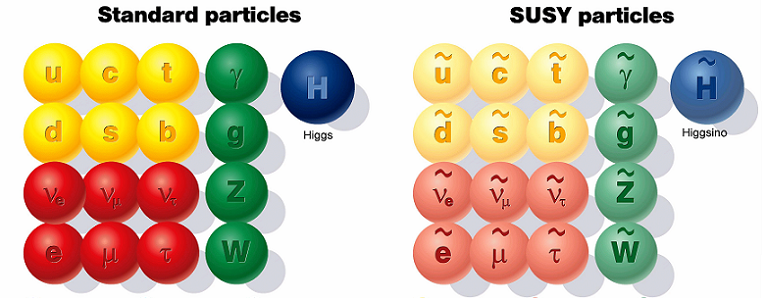
\includegraphics[width=0.85\textwidth]{susy/Particles_MSSM.png}
  \end{center}
  \vskip-0.3cm
  \begin{itemize}
  \item Minimal Supersymmetric Standard Model (MSSM)
    \begin{itemize}
    \item One superpartner to each SM particle (+extended Higgs sector)
    \item R-parity conservation: lightest supersymmetric particle (LSP) is stable
    \end{itemize}
  \end{itemize}
\end{frame}

% ---------------------------------------------------------------------------------
\begin{frame}
  \frametitle{Supersymmetry (SUSY)}
  \begin{columns}
    \begin{column}{0.5\textwidth}
      \centering
      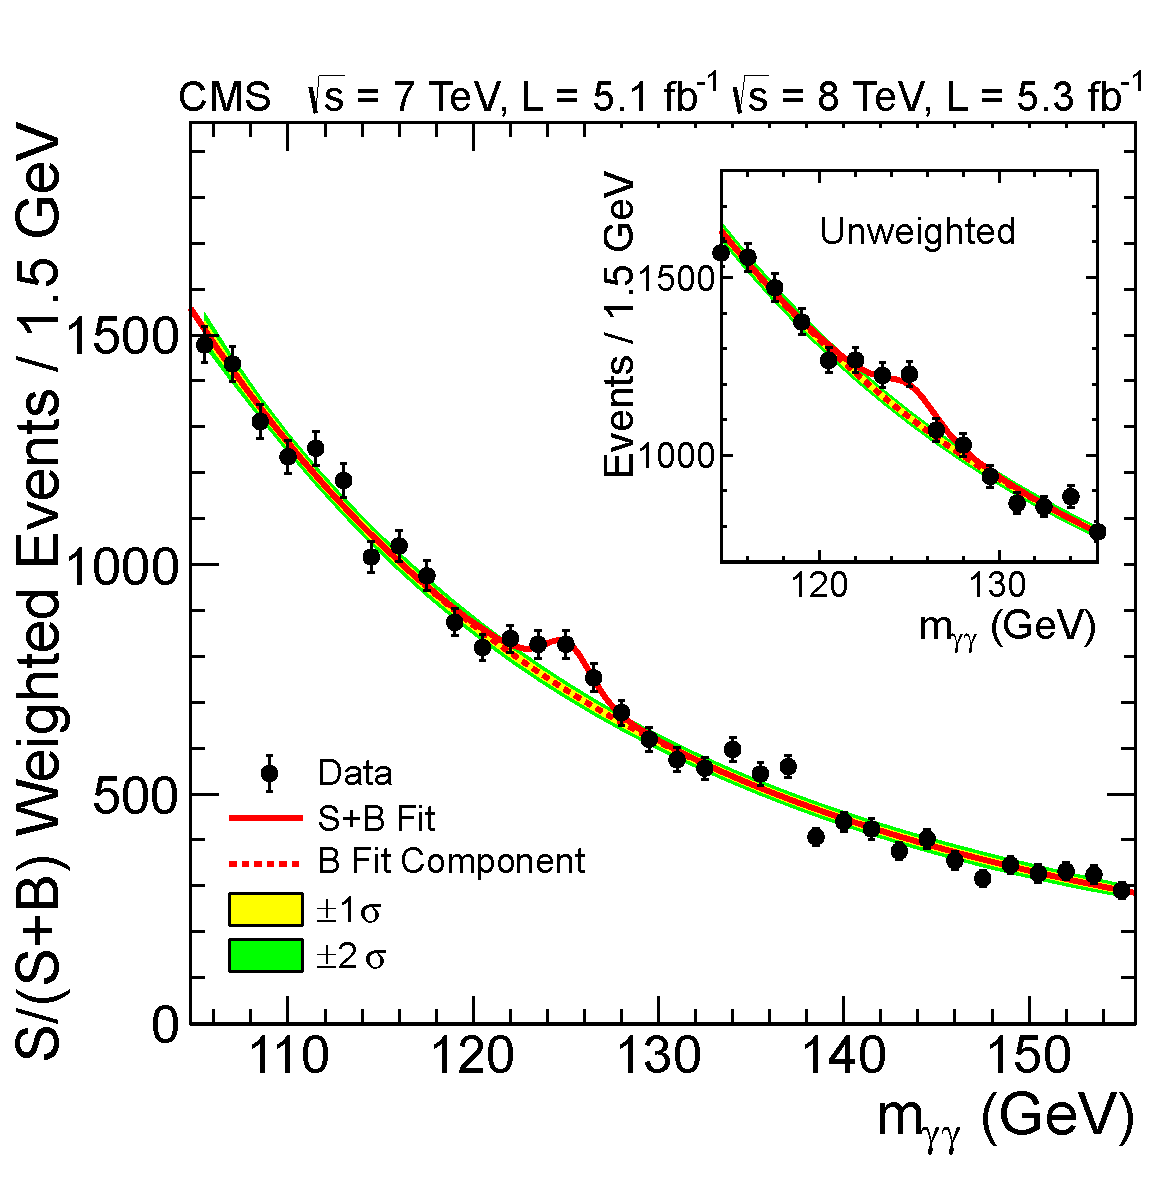
\includegraphics[width=0.49\textwidth]{figures/fig3.pdf}
      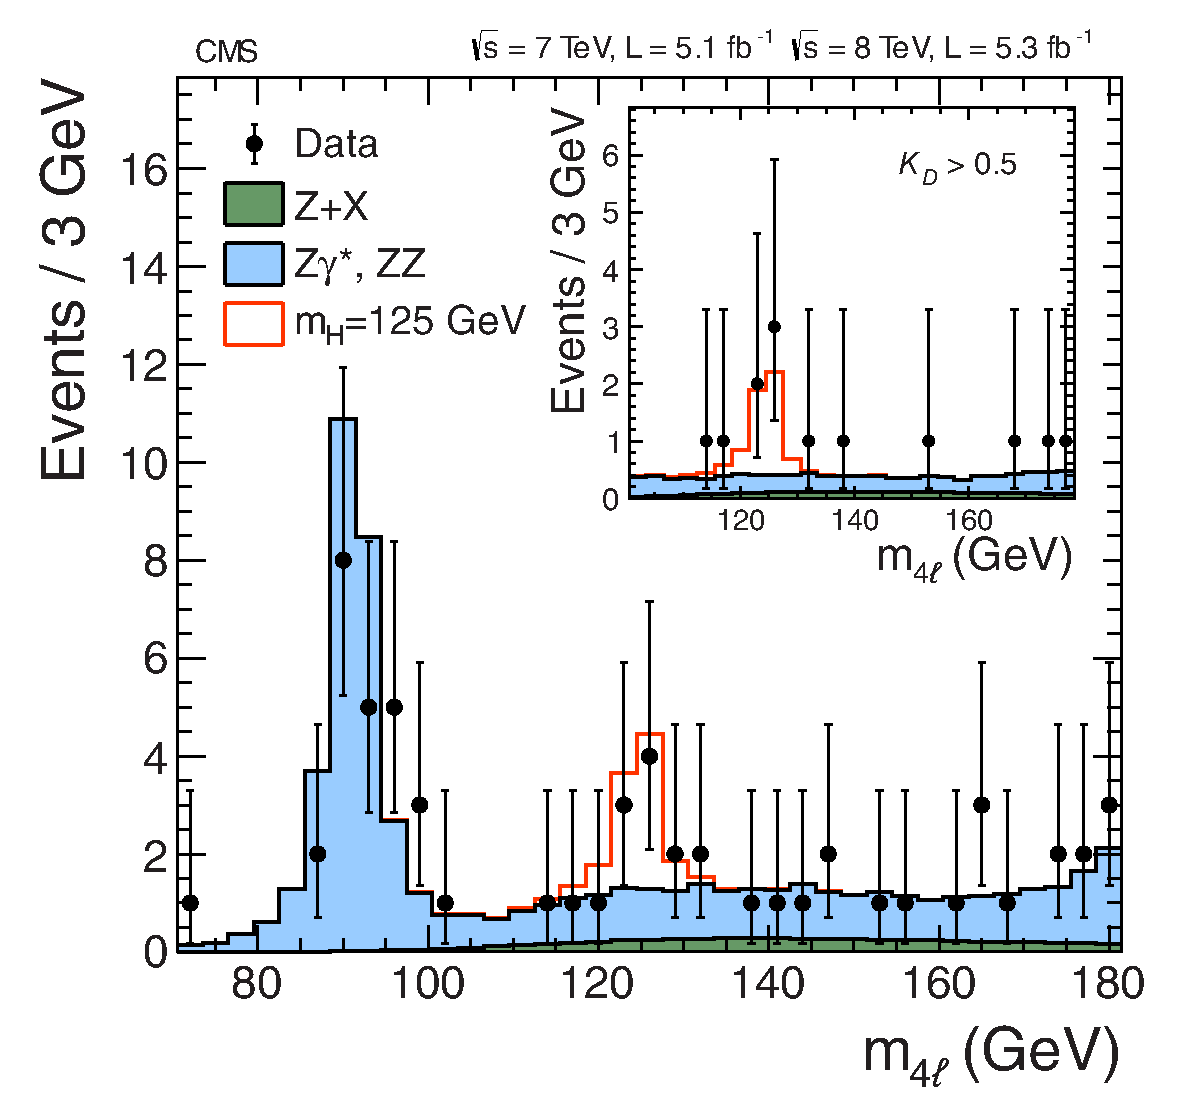
\includegraphics[width=0.51\textwidth]{figures/fig4.pdf}
    \end{column}
    \begin{column}{0.5\textwidth}
      \centering
      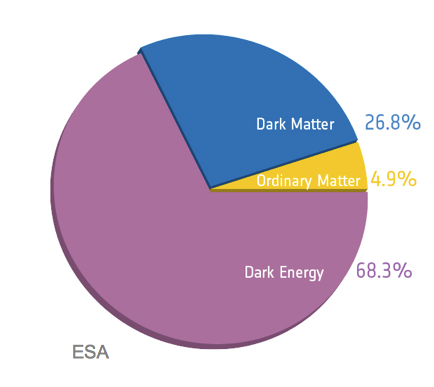
\includegraphics[width=0.7\textwidth]{susy/PlanckUniverse.png}\\
    \end{column}
  \end{columns}    
  \begin{columns}
    \begin{column}{0.49\textwidth}
      \begin{block}{}
        \centering
        \textbf{Solves `Hierarchy Problem' without fine-tuning}
      \end{block}
    \end{column}
    \begin{column}{0.02\textwidth}
    \end{column}
    \begin{column}{0.49\textwidth}
      \begin{block}{}
        \centering
        \textbf{Stable LSP is excellent Dark Matter candidate\emptybox{11pt}}
      \end{block}
    \end{column}
  \end{columns}  
  \vskip0.5cm
  \begin{itemize}
  \item No SUSY particles observed yet
  \item SUSY has to be broken, heavy SUSY particles
  \end{itemize}
\end{frame}


\section{Analysis Motivation}
% --------------------------------------------------
\begin{frame}
  \frametitle{Motivation: Jets + \met Final State}
  \begin{itemize}
  \item Generic, inclusive search for new physics
  \item Motivated by R-parity conserving \susy
    \begin{itemize}
    \item Large cross section for $\tilde{g}\tilde{g}$, $\tilde{g}\tilde{q}$, $\tilde{q}\tilde{q}$ pair-production in many scenarios
    \item Decay into coloured \sm particles and stable LSP
    \end{itemize}
  \end{itemize}
  \begin{columns}
    \begin{column}{0.5\textwidth}
      \centering
      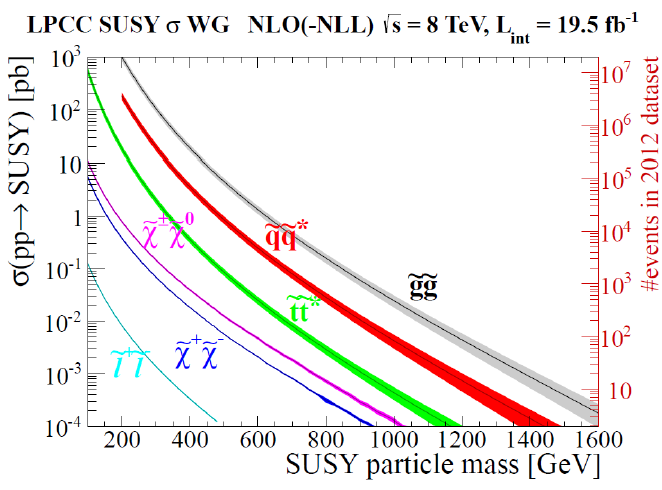
\includegraphics[width=\textwidth]{susy/SUSY-XS-LHC2012-LPCC.png}
    \end{column}
    \begin{column}{0.5\textwidth}
      \only<1>{
        \centering
        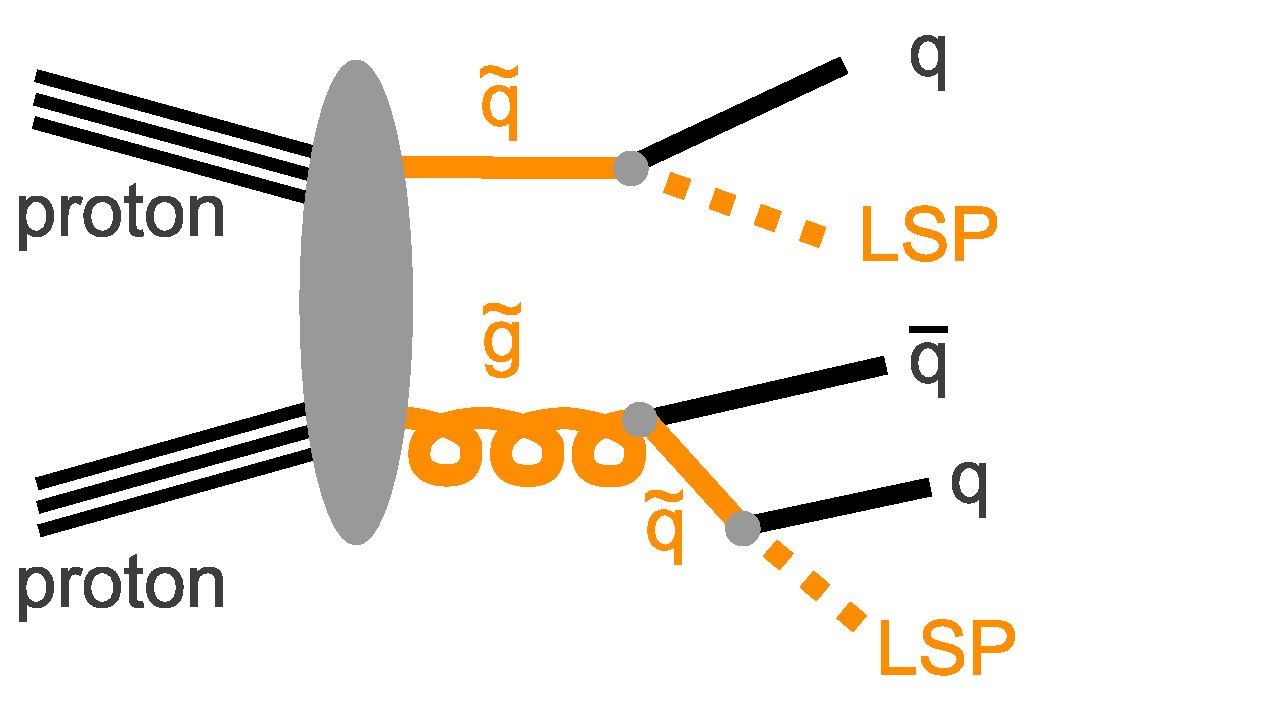
\includegraphics[width=\textwidth]{susy/Sketch_All-HadronicSUSYDiagram_NoText.pdf}
      }
      \only<2->{
        \centering
        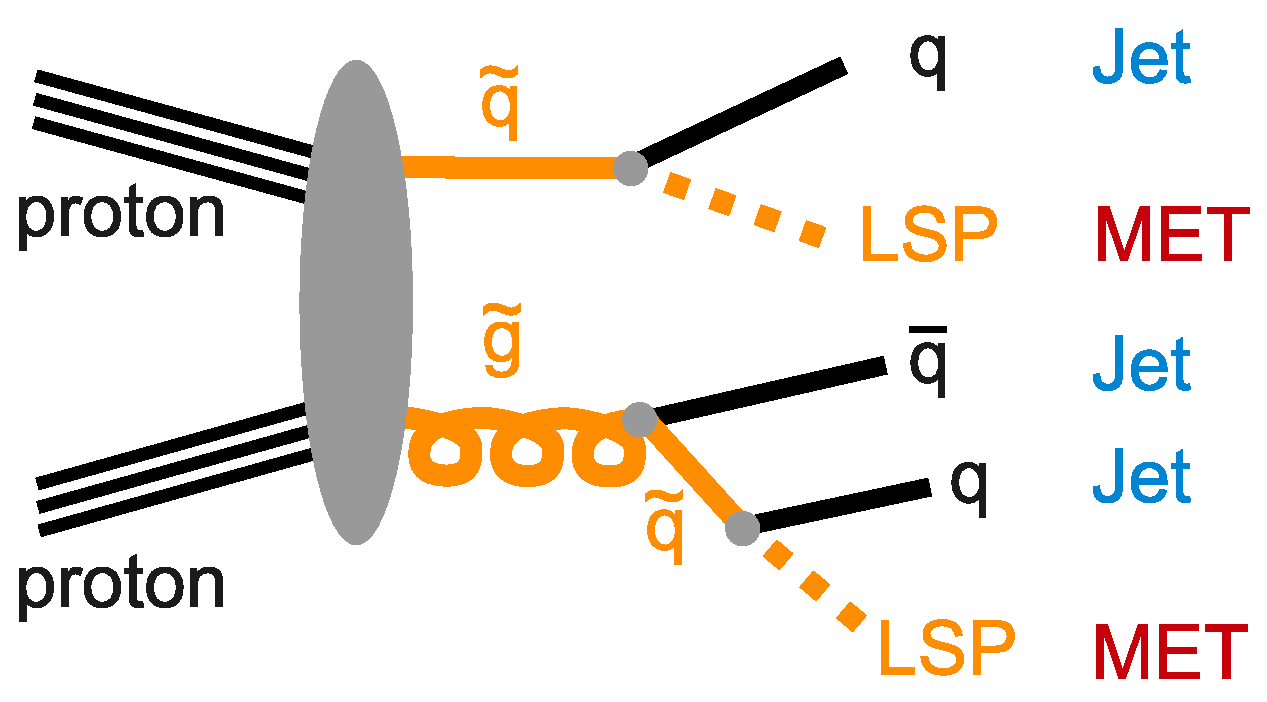
\includegraphics[width=\textwidth]{susy/Sketch_All-HadronicSUSYDiagram.pdf}
      }
    \end{column}
  \end{columns}
  \visible<2->{
    \begin{block}{}
      \centering
      \textbf{Several \textcolor{oochart12}{high-\pt jets} and \textcolor{oochart11}{large missing transverse momentum}}
    \end{block}
  }
\end{frame}

% --------------------------------------------------
\begin{frame}
  \frametitle{Sensitive Variables}
  \begin{columns}
    \begin{column}{0.55\textwidth}
      \centering
      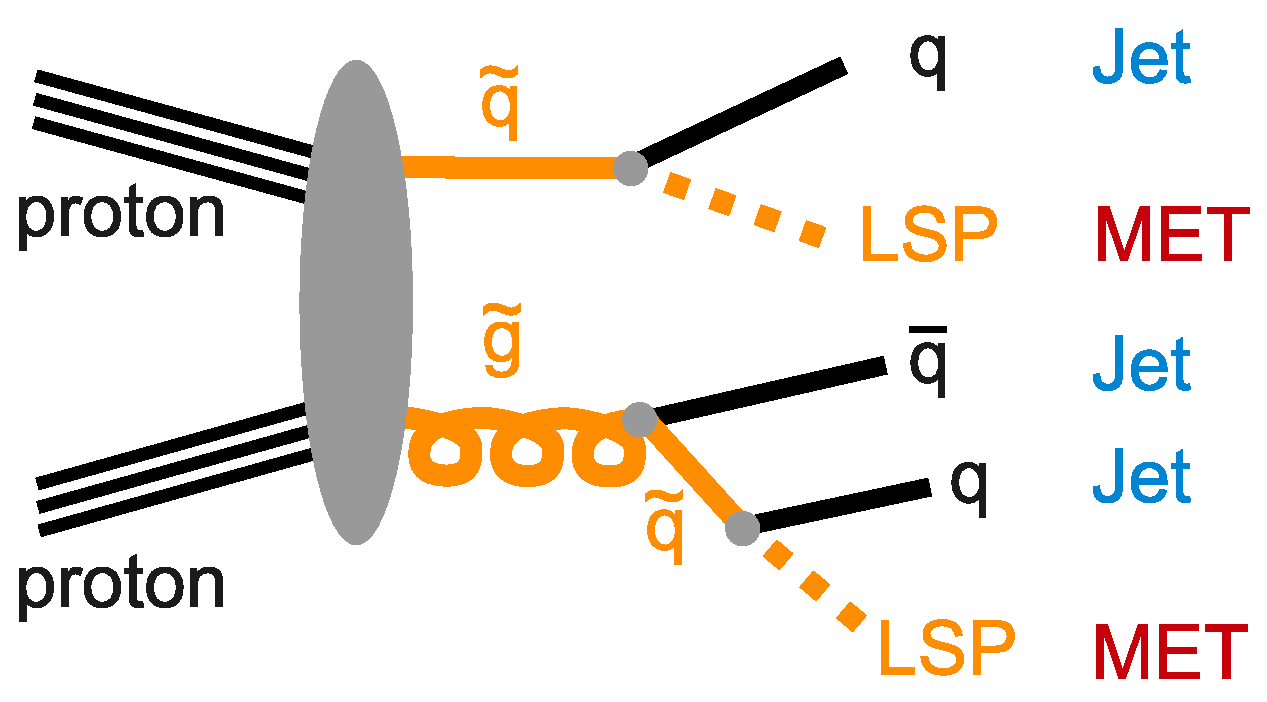
\includegraphics[width=0.9\textwidth]{susy/Sketch_All-HadronicSUSYDiagram.pdf}
    \end{column}
    \begin{column}{0.45\textwidth}
      \begin{block}{}
        \textcolor{oochart12}{Visible energy}
        \begin{equation*}
          \HT = \sum_{\text{jets}} \left|\ptvec\right|
        \end{equation*}
      \end{block}
      \begin{block}{}
        \textcolor{oochart11}{Energy of undetected particles}
        \begin{equation*}
          \MHT = \big|-\sum_{\text{jets}} \ptvec \big|
        \end{equation*}
      \end{block}
    \end{column}
  \end{columns}    
\end{frame}

\section{Event Selection}
% --------------------------------------------------
\begin{frame}
  \frametitle{A SUSY Event?}
  \begin{columns}
    \begin{column}{0.5\textwidth}
      \centering
      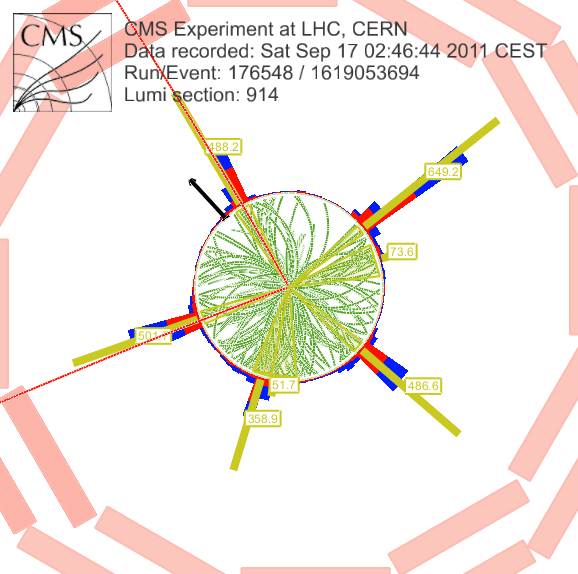
\includegraphics[width=\textwidth]{figures/EvtDisplay_176548_914_1619053694_HT2577_MHT212_RhoPhi.png}
    \end{column}
    \begin{column}{0.5\textwidth}
      \centering
      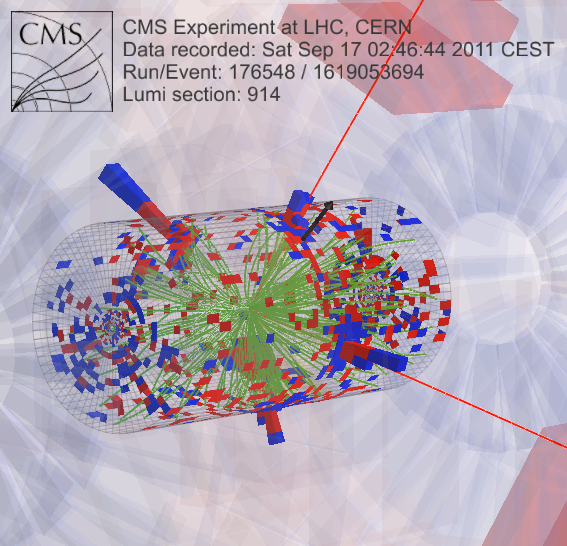
\includegraphics[width=\textwidth]{figures/EvtDisplay_176548_914_1619053694_HT2577_MHT212_3D.png}
    \end{column}
  \end{columns}
\end{frame}

% --------------------------------------------------
\begin{frame}
  \frametitle{The Overwhelming Standard Model}
  \begin{columns}
    \begin{column}{0.45\textwidth}
      \centering
      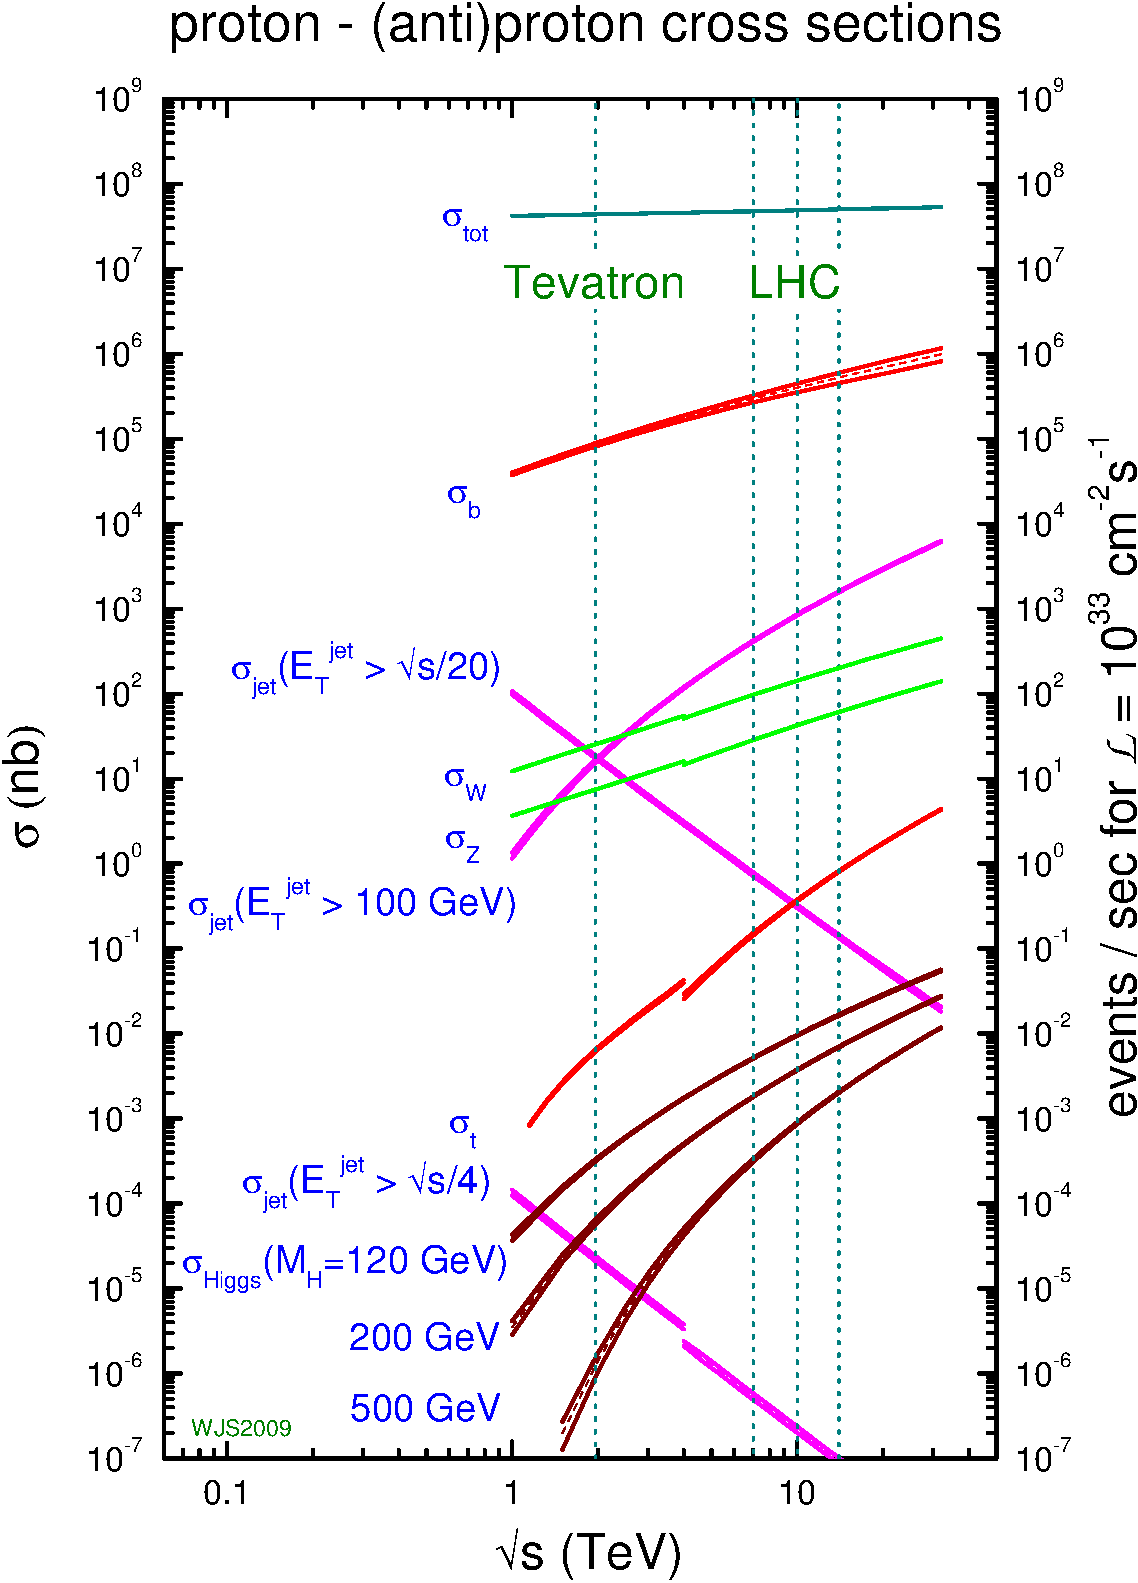
\includegraphics[width=\textwidth]{lhc/crosssections2009_v2.pdf}
    \end{column}
    \begin{column}{0.55\textwidth}
      \begin{itemize}
      \item<2-> SM background processes
        \begin{itemize}
        \item<2-> QCD
        \item<2-> $\text{W}(\rightarrow l\nu)\,+\,\text{jets}$
        \item<2-> $\text{Z}(\rightarrow\nu\bar{\nu})\,+\,\text{jets}$
        \item<2-> \ttbar ($\text{W}(\rightarrow l\nu)$)
        \end{itemize}
      \item<3-> Baseline event selection
        \begin{itemize}
        \item<3-> $\MHT > 200\gev$
        \item<3-> $\ge3$ jets, $HT > 500\gev$
        \item<3-> Veto of events with isolated $e$, $\mu$
        \item<3-> $\Delta\phi(\mht,\text{jet}[1,2,3]) > [0.5,0.5,0.3]$
        \end{itemize}
      \end{itemize}
    \end{column}    
  \end{columns}
\end{frame}

% --------------------------------------------------
\begin{frame}[T]
  \frametitle{After the Baseline Selection}
  \only<1>{
    \begin{columns}
      \begin{column}{0.333\textwidth}
        \centering
        \begin{overpic}[width=\textwidth]{figures/RA2-2012-NoSig__HT__Data_vs_QCD+TTbar+ZJets+WJets__baseline.pdf}
          \put(25,40){\textcolor{white}{\large \bf MC}}
        \end{overpic}
      \end{column}
      \begin{column}{0.333\textwidth}
        \centering
        \begin{overpic}[width=\textwidth]{figures/RA2-2012-NoSig__MHT__Data_vs_QCD+TTbar+ZJets+WJets__baseline.pdf}
          \put(25,40){\textcolor{white}{\large \bf MC}}
        \end{overpic}
      \end{column}
      \begin{column}{0.333\textwidth}
        \centering
        \begin{overpic}[width=\textwidth]{figures/RA2-2012-NoSig__NJets__Data_vs_QCD+TTbar+ZJets+WJets__baseline.pdf}
          \put(25,40){\textcolor{white}{\large \bf MC}}
        \end{overpic}
      \end{column}
    \end{columns}
  }
  \only<2->{
    \begin{columns}
      \begin{column}{0.333\textwidth}
        \centering
        \begin{overpic}[width=\textwidth]{figures/RA2-2012__HT__Data_vs_QCD+TTbar+ZJets+WJets__baseline.pdf}
          \put(25,40){\textcolor{white}{\large \bf MC}}
        \end{overpic}
      \end{column}
      \begin{column}{0.333\textwidth}
        \centering
        \begin{overpic}[width=\textwidth]{figures/RA2-2012__MHT__Data_vs_QCD+TTbar+ZJets+WJets__baseline.pdf}
          \put(25,40){\textcolor{white}{\large \bf MC}}
        \end{overpic}
      \end{column}
      \begin{column}{0.333\textwidth}
        \centering
        \begin{overpic}[width=\textwidth]{figures/RA2-2012__NJets__Data_vs_QCD+TTbar+ZJets+WJets__baseline.pdf}
          \put(25,40){\textcolor{white}{\large \bf MC}}
        \end{overpic}
      \end{column}
    \end{columns}
  }
  \only<1-2>{
    \begin{itemize}
    \item[\solidsquare{black}]<1-2> SM expectation (from MC simulation)
    \item[\solidline{black}]<2> Possible signal (from MC simulation)
    \end{itemize}
    \only<2>{
      \begin{block}{}
        \centering
        \textbf{Precise understanding of background distributions is essential}
      \end{block}
    }
  }
  \only<3->{
    \begin{itemize}
    \item Want sensitivity to many possible signal topologies
    \item 36 search regions in \HT, \MHT, and \NJets on top of baseline selection
    \end{itemize}
  }
  \visible<3->{
    \begin{columns}[T]
      \begin{column}{0.5\textwidth}
        \centering
        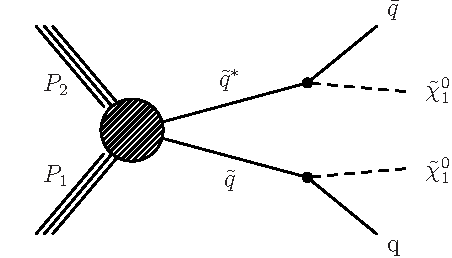
\includegraphics[width=0.7\textwidth]{susy/T2.pdf}\\
        {\small \textbf{high-\MHT} region: high \pt(LSP)}
      \end{column}
      \begin{column}{0.5\textwidth}
        \centering
        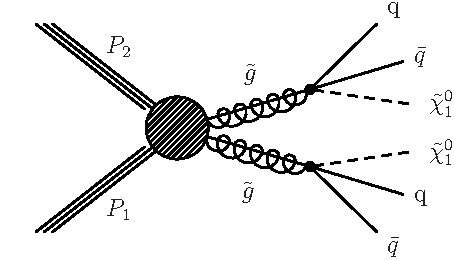
\includegraphics[width=0.7\textwidth]{susy/T1.pdf}\\
        {\small \textbf{low-\MHT} region: many jets}
      \end{column}
    \end{columns}
  }
\end{frame}

\section{Background Prediction}
% --------------------------------------------------
\begin{frame}
  \frametitle{Key Feature of the Analysis}
  \begin{center}
    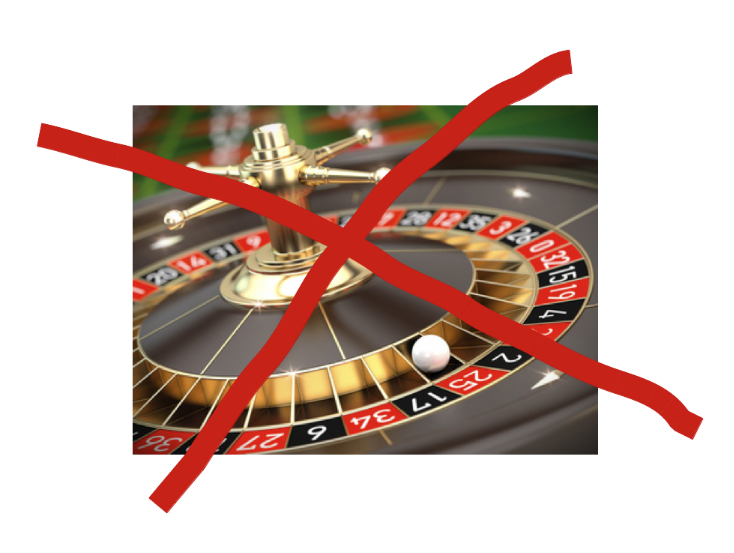
\includegraphics[width=0.6\textwidth]{figures/NoMC.png}
  \end{center}
  \begin{block}{}
    \centering
    \textbf{Measurement of the \sm background from data}
  \end{block}
\end{frame}

% --------------------------------------------------
\begin{frame}
  \frametitle{Data-Based Background Prediction}
  Simple example: $\text{Z}(\rightarrow\nu\bar{\nu})\,+\,\text{jets}$ from $\text{Z}(\rightarrow \mu\mu)\,+\,\text{jets}$ data
  \begin{itemize}
  \item Expect Z decay to be independent of rest of event
  \end{itemize}
  \begin{columns}
    \begin{column}{0.45\textwidth}
      \centering
      \only<1>{
        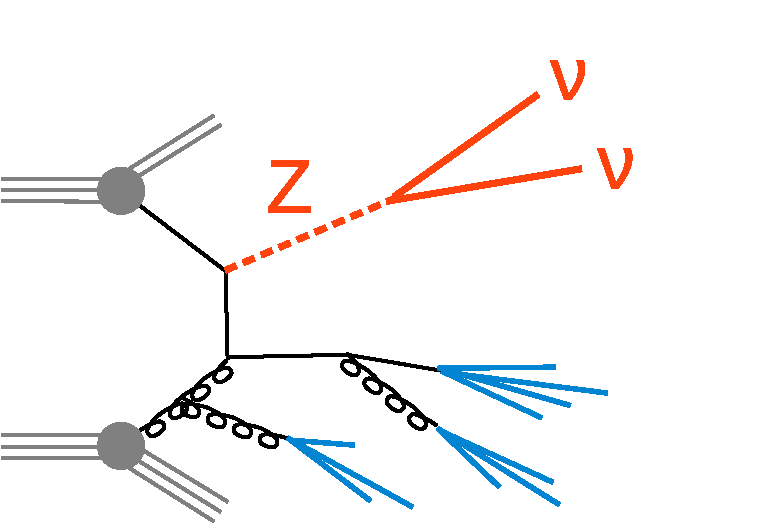
\includegraphics[width=0.9\textwidth]{ra2/Sketch_ZToInv.pdf}\\
      }
      \only<2->{
        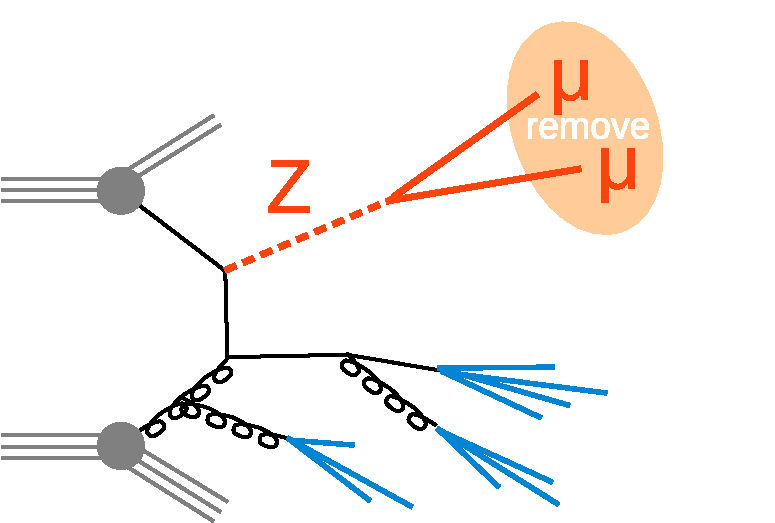
\includegraphics[width=0.9\textwidth]{ra2/Sketch_ZToInvFromMuMu.pdf}\\
      }
    \end{column}
    \begin{column}{0.55\textwidth}
      \begin{block}{}
        \begin{enumerate}
        \item Remove muons from event
        \item Recompute \HT, \MHT, \NJets
        \item Apply baseline selection
        \item Fill distributions for surviving events
        \end{enumerate}
      \end{block}
    \end{column}
  \end{columns}
  \visible<3->{
    \begin{itemize}
    \item[\smiley{}] Advantage: hard-to-predict kinematic properties of event from data
      \begin{itemize}
      \item \NJets and \pt(jets), \ie \HT, \MHT
      \end{itemize}
    \end{itemize}
  }
  \visible<4->{
    \begin{itemize}
    \item Corrections (event weights!)
      \begin{itemize}
      \item BR($\text{Z}\rightarrow \nu\nu$) / BR($\text{Z}\rightarrow \mu\mu$)
      \item Kinematic acceptance and reconstruction efficiency of muons
      \item Trigger efficiency of $\text{Z}(\rightarrow \mu\mu)\,+\,\text{jets}$ events
      \end{itemize}
    \end{itemize}
  }
  \visible<5->{
    \begin{itemize}
    \item[\frownie{}] Drawback: statistical precision, $\text{BR}(\text{Z}\rightarrow \nu\nu) < \text{BR}(\text{Z}\rightarrow \mu\mu)$
    \end{itemize}
  }
\end{frame}

\section{Interpretation of the Results}
% --------------------------------------------------
\begin{frame}
  \frametitle{How to Interpret the Results}
  \begin{center}
    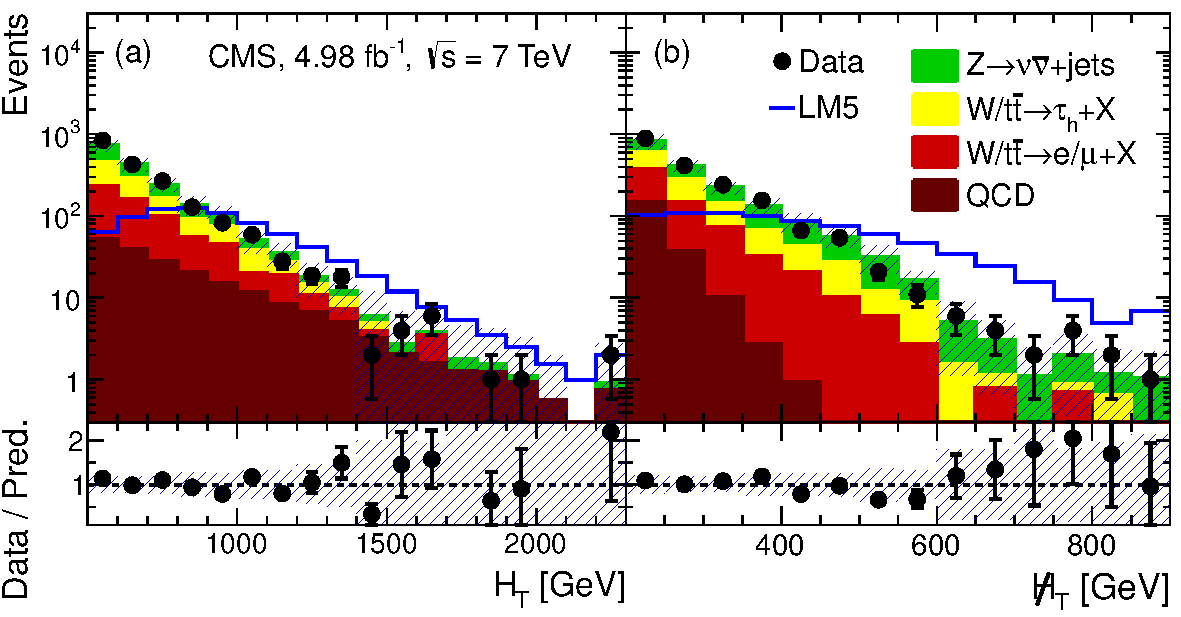
\includegraphics[width=\textwidth]{figures/RA2DataVsEstimatedBkg.pdf}
  \end{center}
\end{frame}

% --------------------------------------------------
\begin{frame}
  \frametitle{95\%-CL Limits on CMSSM Parameters}
  \begin{center}
    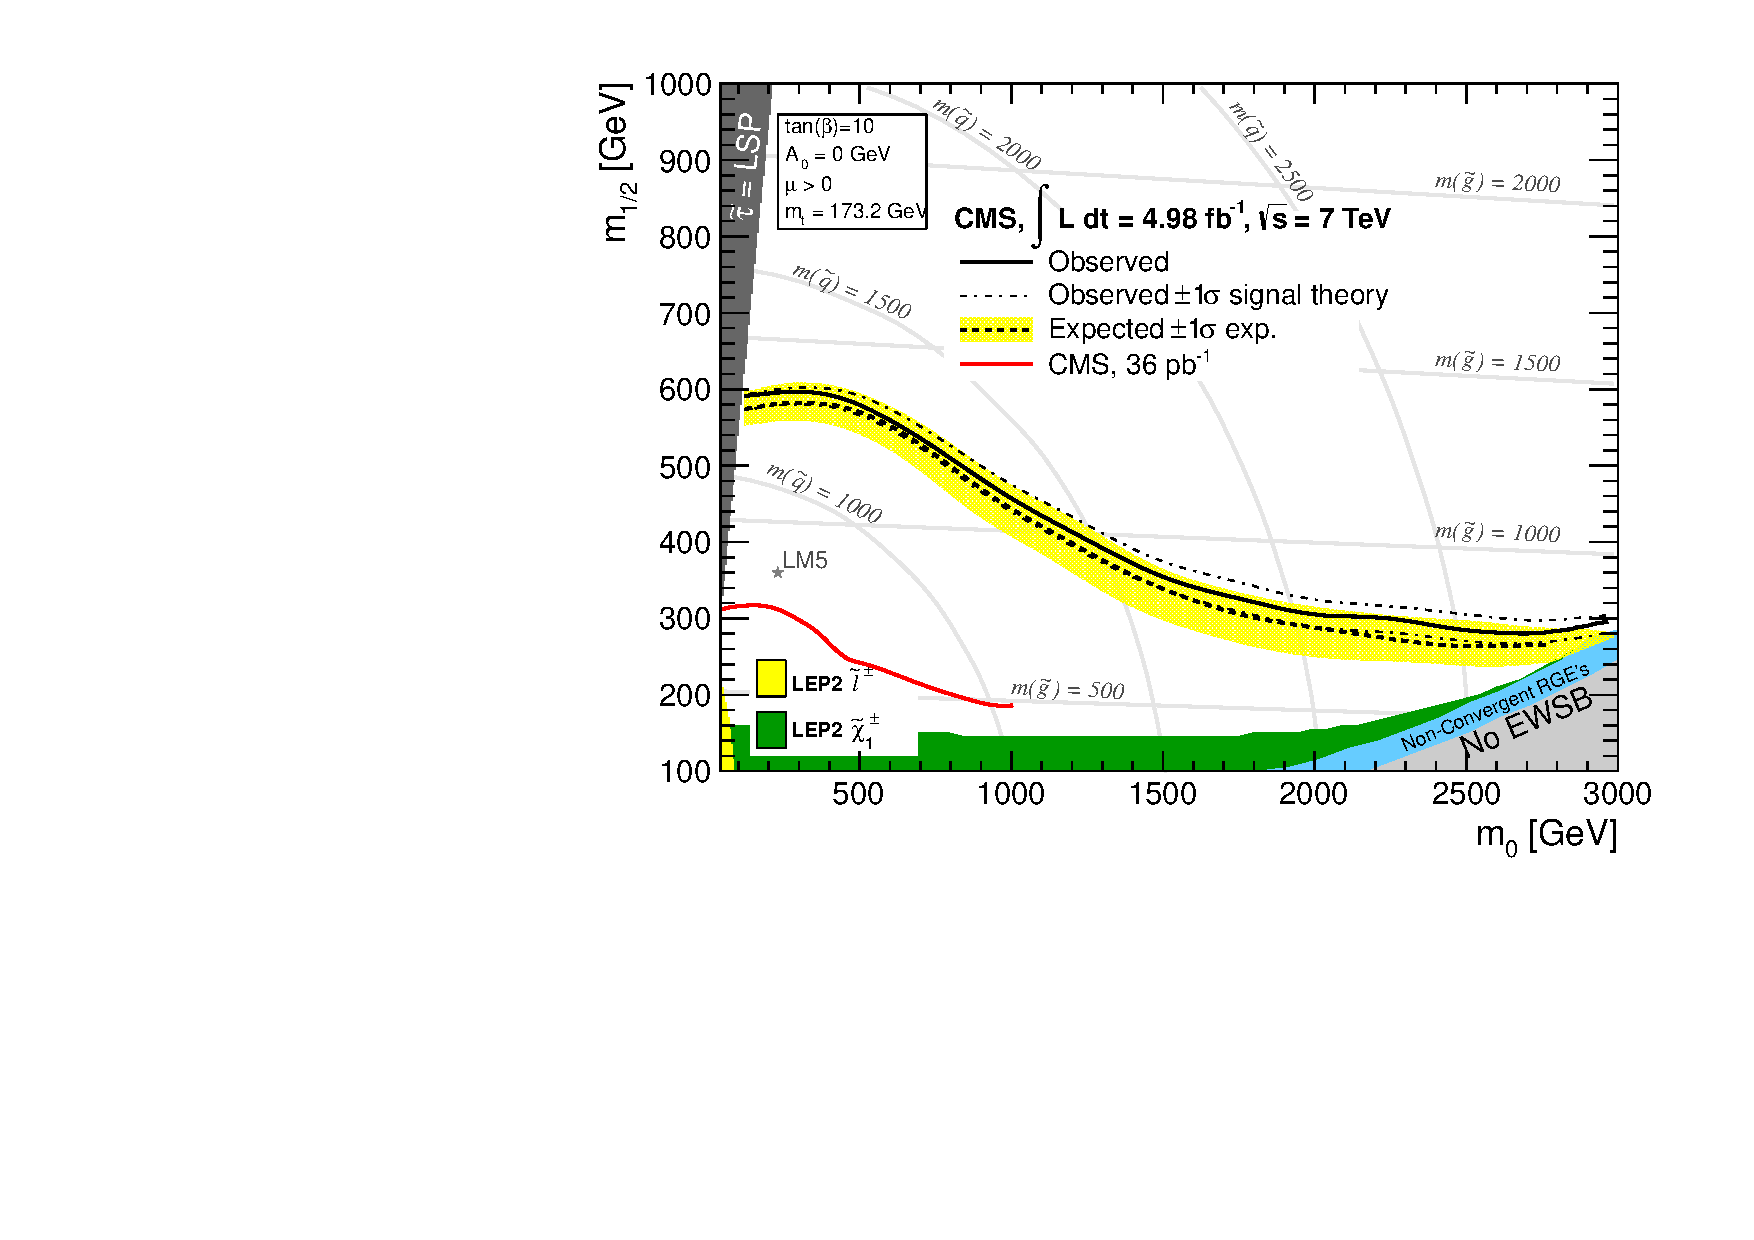
\includegraphics[width=0.9\textwidth]{figures/cMSSM_Mzero_Mhalf_Exclusion.pdf}
  \end{center}
\end{frame}

% --------------------------------------------------
\begin{frame}
  \frametitle{A Word of Warning}
  \begin{columns}
    \begin{column}{0.5\textwidth}
      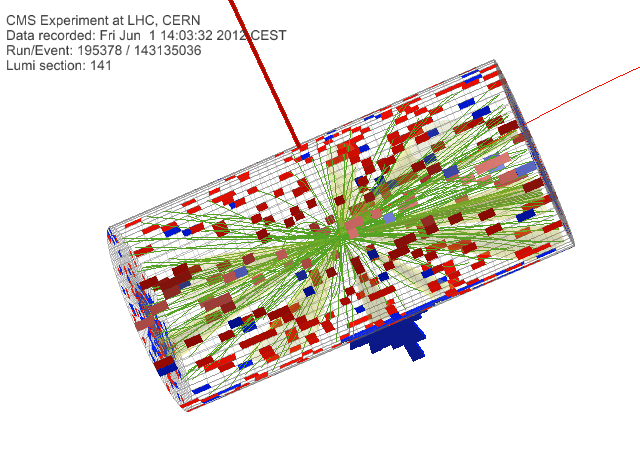
\includegraphics[width=\textwidth]{figures/BeamHalo-195378_143135036_141_3DTower.png}\\
    \end{column}
    \begin{column}{0.5\textwidth}
      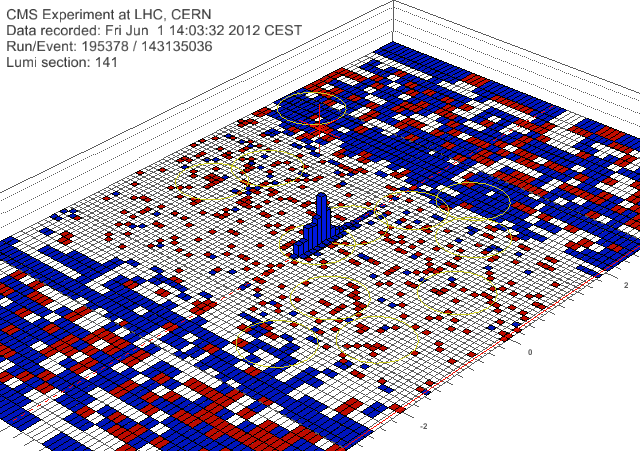
\includegraphics[width=\textwidth]{figures/BeamHalo-195378_143135036_141_Lego.png}\\
    \end{column}
  \end{columns}
  \begin{itemize}
  \item Searches typically look in extreme phase-space regions, \eg high \MHT
  \item Fake signal events due to rare effects become extremely important
    \begin{itemize}
    \item Misreconstruction, detector noise, dead channels
    \item Beam-background events
    \end{itemize}
  \end{itemize}
  \begin{block}{}
    \center
    \textbf{Careful selection of high-quality events is essential}
  \end{block}
\end{frame}

\section{The Exercise}
% --------------------------------------------------
\begin{frame}[t]
  \frametitle{The Exercise}
  \url{https://twiki.cern.ch/twiki/bin/viewauth/CMS/SUSYExersice2015BARI}
  \vskip0.5cm
  \begin{itemize}
  \item First Part:
    \begin{itemize}
    \item Investigating the properties of data, SM background, and signal processes
    \item Understanding the event selection
    \item Understanding the data-based background prediction methods
    \end{itemize}
  \item Second Part:
  \begin{itemize}
    \item Prediction of the \wpj and \ttbar backgrounds
    \item Combining the results and comparing to data
    \end{itemize}
    \item End:
    \begin{itemize}
    \item Preparing the presentation
    \item Result presentation
    \end{itemize}
  \end{itemize}
\end{frame}

% --------------------------------------------------




%\setcounter{framenumber}{18}

\end{document}
